\documentclass{standalone}
\usepackage{tikz}
\usetikzlibrary{patterns, positioning}


\begin{document}
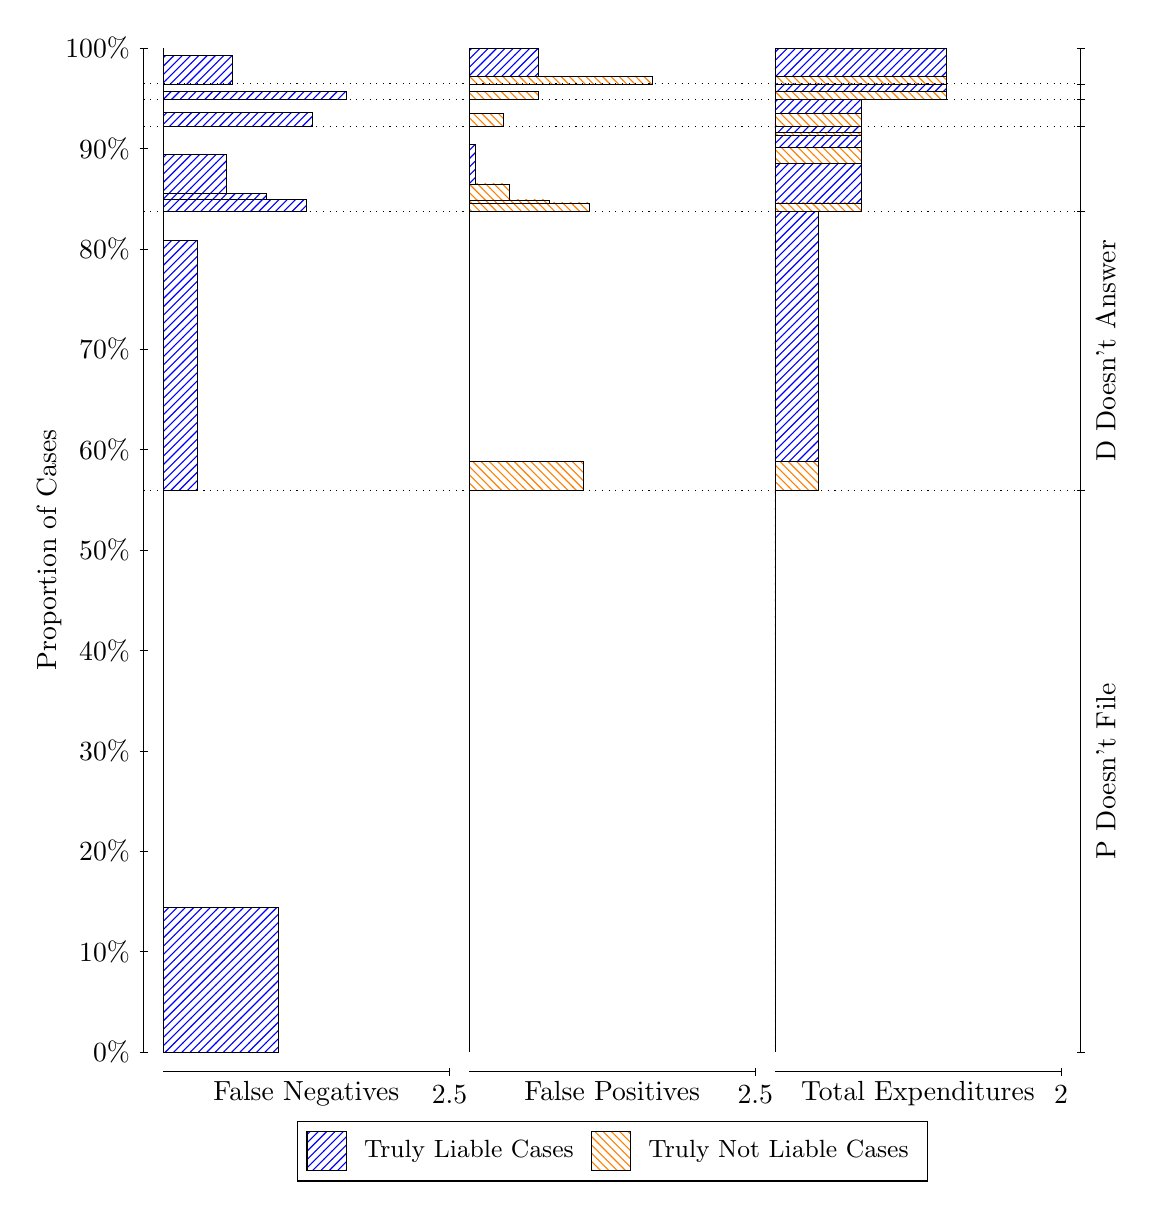
\begin{tikzpicture}
\draw[black, very thin] (1.5,1.75) -- (1.5,14.5);
\node[rotate=90, text=black, anchor=center] at (0.3, 8.125) {Proportion of Cases};
\draw[black, very thin] (1.45,1.75) -- (1.55,1.75);
\node[text=black, anchor=east] at (1.45, 1.75) {0\%};
\draw[black, very thin] (1.45,3.025) -- (1.55,3.025);
\node[text=black, anchor=east] at (1.45, 3.025) {10\%};
\draw[black, very thin] (1.45,4.3) -- (1.55,4.3);
\node[text=black, anchor=east] at (1.45, 4.3) {20\%};
\draw[black, very thin] (1.45,5.575) -- (1.55,5.575);
\node[text=black, anchor=east] at (1.45, 5.575) {30\%};
\draw[black, very thin] (1.45,6.85) -- (1.55,6.85);
\node[text=black, anchor=east] at (1.45, 6.85) {40\%};
\draw[black, very thin] (1.45,8.125) -- (1.55,8.125);
\node[text=black, anchor=east] at (1.45, 8.125) {50\%};
\draw[black, very thin] (1.45,9.4) -- (1.55,9.4);
\node[text=black, anchor=east] at (1.45, 9.4) {60\%};
\draw[black, very thin] (1.45,10.675) -- (1.55,10.675);
\node[text=black, anchor=east] at (1.45, 10.675) {70\%};
\draw[black, very thin] (1.45,11.95) -- (1.55,11.95);
\node[text=black, anchor=east] at (1.45, 11.95) {80\%};
\draw[black, very thin] (1.45,13.225) -- (1.55,13.225);
\node[text=black, anchor=east] at (1.45, 13.225) {90\%};
\draw[black, very thin] (1.45,14.5) -- (1.55,14.5);
\node[text=black, anchor=east] at (1.45, 14.5) {100\%};

\draw[black, very thin] (13.4,1.75) -- (13.4,14.5);
\draw[black, very thin] (13.35,1.75) -- (13.45,1.75);
\node[anchor=west] at (13.35, 1.75) {};
\draw[black, very thin] (13.35,8.8829) -- (13.45,8.8829);
\node[anchor=west] at (13.35, 8.8829) {};
\draw[black, very thin] (13.35,12.421) -- (13.45,12.421);
\node[anchor=west] at (13.35, 12.421) {};
\draw[black, very thin] (13.35,13.509) -- (13.45,13.509);
\node[anchor=west] at (13.35, 13.509) {};
\draw[black, very thin] (13.35,13.851) -- (13.45,13.851);
\node[anchor=west] at (13.35, 13.851) {};
\draw[black, very thin] (13.35,14.044) -- (13.45,14.044);
\node[anchor=west] at (13.35, 14.044) {};
\draw[black, very thin] (13.35,14.5) -- (13.45,14.5);
\node[anchor=west] at (13.35, 14.5) {};

\draw[black, very thin, pattern color=blue, pattern=north east lines] (1.75,1.75) rectangle (3.2033,3.5845);
\draw[black, very thin, pattern color=orange, pattern=north west lines] (1.75,3.5845) rectangle (1.75,8.8829);
\draw[black, very thin, pattern color=blue, pattern=north east lines] (1.75,8.8829) rectangle (2.186,12.057);
\draw[black, very thin, pattern color=orange, pattern=north west lines] (1.75,12.057) rectangle (1.75,12.421);
\draw[black, very thin, pattern color=blue, pattern=north east lines] (1.75,12.421) rectangle (3.5667,12.577);
\draw[black, very thin, pattern color=blue, pattern=north east lines] (1.75,12.577) rectangle (3.058,12.656);
\draw[black, very thin, pattern color=blue, pattern=north east lines] (1.75,12.656) rectangle (2.5493,13.153);
\draw[black, very thin, pattern color=orange, pattern=north west lines] (1.75,13.153) rectangle (1.75,13.509);
\draw[black, very thin, pattern color=blue, pattern=north east lines] (1.75,13.509) rectangle (3.6393,13.686);
\draw[black, very thin, pattern color=orange, pattern=north west lines] (1.75,13.686) rectangle (1.75,13.851);
\draw[black, very thin, pattern color=blue, pattern=north east lines] (1.75,13.851) rectangle (4.0753,13.948);
\draw[black, very thin, pattern color=orange, pattern=north west lines] (1.75,13.948) rectangle (1.75,14.044);
\draw[black, very thin, pattern color=blue, pattern=north east lines] (1.75,14.044) rectangle (2.622,14.403);
\draw[black, very thin, pattern color=orange, pattern=north west lines] (1.75,14.403) rectangle (1.75,14.5);
\draw[black, very thin, pattern color=orange, pattern=north west lines] (5.6333,1.75) rectangle (5.6333,7.0484);
\draw[black, very thin, pattern color=blue, pattern=north east lines] (5.6333,7.0484) rectangle (5.6333,8.8829);
\draw[black, very thin, pattern color=orange, pattern=north west lines] (5.6333,8.8829) rectangle (7.0867,9.247);
\draw[black, very thin, pattern color=blue, pattern=north east lines] (5.6333,9.247) rectangle (5.6333,12.421);
\draw[black, very thin, pattern color=orange, pattern=north west lines] (5.6333,12.421) rectangle (7.1593,12.533);
\draw[black, very thin, pattern color=orange, pattern=north west lines] (5.6333,12.533) rectangle (6.6507,12.572);
\draw[black, very thin, pattern color=orange, pattern=north west lines] (5.6333,12.572) rectangle (6.142,12.776);
\draw[black, very thin, pattern color=blue, pattern=north east lines] (5.6333,12.776) rectangle (5.706,13.274);
\draw[black, very thin, pattern color=blue, pattern=north east lines] (5.6333,13.274) rectangle (5.6333,13.509);
\draw[black, very thin, pattern color=orange, pattern=north west lines] (5.6333,13.509) rectangle (6.0693,13.674);
\draw[black, very thin, pattern color=blue, pattern=north east lines] (5.6333,13.674) rectangle (5.6333,13.851);
\draw[black, very thin, pattern color=orange, pattern=north west lines] (5.6333,13.851) rectangle (6.5053,13.947);
\draw[black, very thin, pattern color=blue, pattern=north east lines] (5.6333,13.947) rectangle (5.6333,14.044);
\draw[black, very thin, pattern color=orange, pattern=north west lines] (5.6333,14.044) rectangle (7.9587,14.141);
\draw[black, very thin, pattern color=blue, pattern=north east lines] (5.6333,14.141) rectangle (6.5053,14.5);
\draw[black, very thin, pattern color=orange, pattern=north west lines] (9.5167,1.75) rectangle (9.5167,7.0484);
\draw[black, very thin, pattern color=blue, pattern=north east lines] (9.5167,7.0484) rectangle (9.5167,8.8829);
\draw[black, very thin, pattern color=orange, pattern=north west lines] (9.5167,8.8829) rectangle (10.062,9.247);
\draw[black, very thin, pattern color=blue, pattern=north east lines] (9.5167,9.247) rectangle (10.062,12.421);
\draw[black, very thin, pattern color=orange, pattern=north west lines] (9.5167,12.421) rectangle (10.607,12.533);
\draw[black, very thin, pattern color=blue, pattern=north east lines] (9.5167,12.533) rectangle (10.607,13.031);
\draw[black, very thin, pattern color=orange, pattern=north west lines] (9.5167,13.031) rectangle (10.607,13.235);
\draw[black, very thin, pattern color=blue, pattern=north east lines] (9.5167,13.235) rectangle (10.607,13.391);
\draw[black, very thin, pattern color=orange, pattern=north west lines] (9.5167,13.391) rectangle (10.607,13.43);
\draw[black, very thin, pattern color=blue, pattern=north east lines] (9.5167,13.43) rectangle (10.607,13.509);
\draw[black, very thin, pattern color=orange, pattern=north west lines] (9.5167,13.509) rectangle (10.607,13.674);
\draw[black, very thin, pattern color=blue, pattern=north east lines] (9.5167,13.674) rectangle (10.607,13.851);
\draw[black, very thin, pattern color=orange, pattern=north west lines] (9.5167,13.851) rectangle (11.697,13.947);
\draw[black, very thin, pattern color=blue, pattern=north east lines] (9.5167,13.947) rectangle (11.697,14.044);
\draw[black, very thin, pattern color=orange, pattern=north west lines] (9.5167,14.044) rectangle (11.697,14.141);
\draw[black, very thin, pattern color=blue, pattern=north east lines] (9.5167,14.141) rectangle (11.697,14.5);
\draw[black, dotted] (1.5,8.8829) -- (13.4,8.8829);
\draw[black, dotted] (1.5,12.421) -- (13.4,12.421);
\draw[black, dotted] (1.5,13.509) -- (13.4,13.509);
\draw[black, dotted] (1.5,13.851) -- (13.4,13.851);
\draw[black, dotted] (1.5,14.044) -- (13.4,14.044);
\draw[black, very thin] (1.75,1.5) -- (5.3833,1.5);
\node[text=black, anchor=north] at (3.5667, 1.5) {False Negatives};
\draw[black, very thin] (5.3833,1.45) -- (5.3833,1.55);
\node[text=black, anchor=north] at (5.3833, 1.45) {2.5};

\draw[black, very thin] (5.6333,1.5) -- (9.2667,1.5);
\node[text=black, anchor=north] at (7.45, 1.5) {False Positives};
\draw[black, very thin] (9.2667,1.45) -- (9.2667,1.55);
\node[text=black, anchor=north] at (9.2667, 1.45) {2.5};

\draw[black, very thin] (9.5167,1.5) -- (13.15,1.5);
\node[text=black, anchor=north] at (11.333, 1.5) {Total Expenditures};
\draw[black, very thin] (13.15,1.45) -- (13.15,1.55);
\node[text=black, anchor=north] at (13.15, 1.45) {2};

\node[text=black, centered, rotate=90] at (13.72, 5.3164) {P Doesn't File};
\node[text=black, centered, rotate=90] at (13.72, 10.652) {D Doesn't Answer};





\draw (7.449999999999999,1.5) node[draw=none] (baseCoordinate) {};
\begin{scope}[align=center]
        \matrix[scale=0.5, draw=black, below=0.5cm of baseCoordinate, nodes={draw}, column sep=0.1cm]{
            \node[rectangle, draw, minimum width=0.5cm, minimum height=0.5cm, pattern color=blue, pattern=north east lines] {}; &
            \node[draw=none, font=\small, text=black] (B) {Truly Liable Cases}; &
            \node[rectangle, draw, minimum width=0.5cm, minimum height=0.5cm, pattern color=orange, pattern=north west lines] {}; &
            \node[draw=none, font=\small, text=black] (B) {Truly Not Liable Cases}; \\
            };
\end{scope}

\end{tikzpicture}
\end{document}